\paragraph{Overall System}
% Introduce the layered architecture
We propose building a layered system where each piece of the
funcionality of the overall application is built into one layer of the
overall design.

% Give overview of why this is a good idea.  
This design gives us the ability to build the riskiest, most difficult
pieces of functionality early, while slowly building up to an
application taht is usable.
It also allows us to parallel path much of the development of the
overall system.
One person can easily be working on one layer of the system without
impacting other layers, as long as interfaces between layers are well
designed and documented.

The other primary advantage of the layered model detailed in the
following sections is that it makes validation possible at each layer
of the model.
% TODO: what section?
As we will get into in the following sections, the overall application
will need to be validated as it is built, for the accuracy of its NLP
algorithms, the usefullness of its suggestions, and the
user-friendlyness of it's UI

% TODO: figure ref doesn't seem to be resolving correctly
See figure \ref{sec:system-design:fig:design} for a detailed
breakdown of the overall system design.
The arrows in this diagram represent the flow of information from one
layer to the next.
Notice how no layer communicates with anything past its surrounding layers.

\begin{figure*}[h]
\label{sec:system-design:fig:design}
\caption{Visualization of layered architecture}
\centering
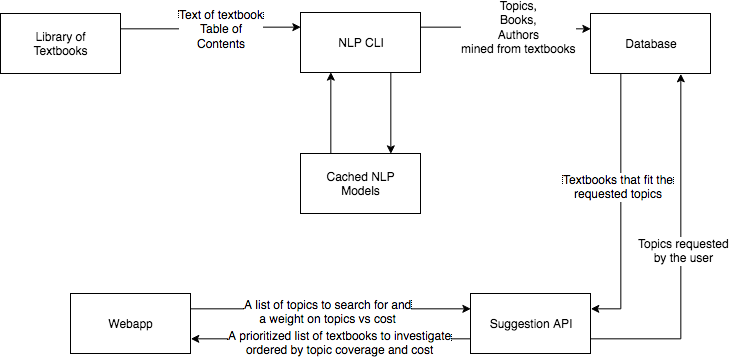
\includegraphics[width=\textwidth]{SystemDesign}
\end{figure*}

\paragraph{Textbook Library}
% TODO: should we detail the textbook library as a part of the overall system?

\paragraph{NLP Algorithm}
% Talk about the design of the NLP algorithms
The ``lowest'' level of the stack we have designed is the suggestion
algorithms.
This layer has the responsibility of identifying the topis found in
textbooks using trained models.
Because all modern topic modeling algorithms are extremely slow to
run, analysis can not be done in real-time.
To work around that, we propose buildign a command-line application
that could be scheduled on a server to run on some kind of regular
interval and set against some external textbook parsing API.  
See section \ref{sec:cli-design} for a more detailed breakdown than
this overview.

\paragraph{Database}
% Talk about the design of the database
The database sits above the NLP algorithms, but below the rest of the
stack.
Its purpose is to hold the topics, textbooks, and author information
mined from our external API.  
To house this information, we have assembled a database using the
Python library Peewee as an ORM.
When run, Peewee will build out the tables listed in figure \ref{sec:system-design:fig:erd}.
The app proposed will use the database as a repository from which to
make suggestions rather than natively running the NLP algorithms,
which should help to improve the performance of the overall app.

\begin{figure*}[h]
\label{sec:system-design:fig:erd}
\caption{ERD of Proposed Database}
\centering
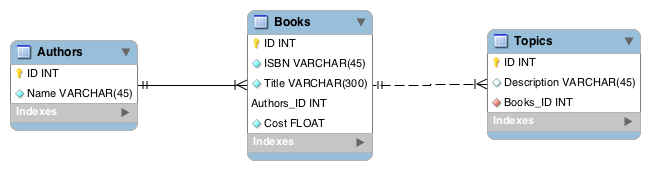
\includegraphics[width=\textwidth]{ERD}
\end{figure*}

\paragraph{Suggestion Algorithm}
% Talk about the design of the algorithms API
The suggestion layer is the last layer of the application before the
interface itself.
To make suggestions, the team intends to build out a REST API built on
top of the database previously discussed.
The API should accept a list of topics to search for along with two
weights: one for the wieght of topic coverage and one for weight of
cost.

The weights serve as tuning parameters and may or may not be displayed
to the end-users.
The weights are them multiplied by their respective parameters and
summed to come to a final priority number, which can then be
considered a measure of the ``fitness'' of a particular textbook for
use, where larger numbers are more fit.
The fitness numbers should also be normalized to a scale between 0 and
1, so that the ``fitness'' of different searches could be compared in
a meaningful way.

The proposed formula for calculating the priority of a suggestion is
detailed in equation \ref{sec:system-design:eq:priority}.


\begin{align}
P_i &= a \times num\_topics_i + (b \times max(cost) - cost_i) \label{sec:system-design:eq:priority}
\end{align}

\paragraph{Web App}
% Talk about the design of the webapp
The final componenet in this proposed architecture is the user
interface.
For the purpose of this project, the team proposes building a simple
webapp using AngularJS.
In this design, the actual web app needs to do very little; it is
merely acting as an interface to the previously mentioned API.
It does not need to directly connect to a database or to perform
complex calculations, it simply needs to provide a simple, easy way to
input a set of search topics and to display the results of the REST
API to the users.

AngularJS is well positioned to be useful in this situation.
It provides convenient APIs for the display and manipulation of
complex interfaces, without providing significant bloat to the
application stack duplicating the features of the previous components.
It is also structured as a model-view-controller system, so our
manipulation of the REST api can be well and cleanly separated from
the presentation, allowing us to develop other applications easily in
the future.  

%%% Local Variables:
%%% mode: latex
%%% TeX-master: "../../main"
%%% End:
